\documentclass[12pt,a4paper]{article}

%\usepackage[left=1.5cm,right=1.5cm,top=1cm,bottom=2cm]{geometry}
\usepackage[in, plain]{fullpage}
\usepackage{array}
\usepackage{../../../pas-math}
\usepackage{../../../moncours}


%\usepackage{pas-cours}
%-------------------------------------------------------------------------------
%          -Packages nécessaires pour écrire en Français et en UTF8-
%-------------------------------------------------------------------------------
\usepackage[utf8]{inputenc}
\usepackage[frenchb]{babel}
\usepackage[T1]{fontenc}
\usepackage{lmodern}
\usepackage{textcomp}



%-------------------------------------------------------------------------------

%-------------------------------------------------------------------------------
%                          -Outils de mise en forme-
%-------------------------------------------------------------------------------
\usepackage{hyperref}
\hypersetup{pdfstartview=XYZ}
%\usepackage{enumerate}
\usepackage{graphicx}
\usepackage{multicol}
\usepackage{tabularx}
\usepackage{multirow}


\usepackage{anysize} %%pour pouvoir mettre les marges qu'on veut
%\marginsize{2.5cm}{2.5cm}{2.5cm}{2.5cm}

\usepackage{indentfirst} %%pour que les premier paragraphes soient aussi indentés
\usepackage{verbatim}
\usepackage{enumitem}
\usepackage[usenames,dvipsnames,svgnames,table]{xcolor}

\usepackage{variations}

%-------------------------------------------------------------------------------


%-------------------------------------------------------------------------------
%                  -Nécessaires pour écrire des mathématiques-
%-------------------------------------------------------------------------------
\usepackage{amsfonts}
\usepackage{amssymb}
\usepackage{amsmath}
\usepackage{amsthm}
\usepackage{tikz}
\usepackage{xlop}
%-------------------------------------------------------------------------------



%-------------------------------------------------------------------------------


%-------------------------------------------------------------------------------
%                    - Mise en forme avancée
%-------------------------------------------------------------------------------

\usepackage{ifthen}
\usepackage{ifmtarg}


\newcommand{\ifTrue}[2]{\ifthenelse{\equal{#1}{true}}{#2}{$\qquad \qquad$}}

%-------------------------------------------------------------------------------

%-------------------------------------------------------------------------------
%                     -Mise en forme d'exercices-
%-------------------------------------------------------------------------------
%\newtheoremstyle{exostyle}
%{\topsep}% espace avant
%{\topsep}% espace apres
%{}% Police utilisee par le style de thm
%{}% Indentation (vide = aucune, \parindent = indentation paragraphe)
%{\bfseries}% Police du titre de thm
%{.}% Signe de ponctuation apres le titre du thm
%{ }% Espace apres le titre du thm (\newline = linebreak)
%{\thmname{#1}\thmnumber{ #2}\thmnote{. \normalfont{\textit{#3}}}}% composants du titre du thm : \thmname = nom du thm, \thmnumber = numéro du thm, \thmnote = sous-titre du thm

%\theoremstyle{exostyle}
%\newtheorem{exercice}{Exercice}
%
%\newenvironment{questions}{
%\begin{enumerate}[\hspace{12pt}\bfseries\itshape a.]}{\end{enumerate}
%} %mettre un 1 à la place du a si on veut des numéros au lieu de lettres pour les questions 
%-------------------------------------------------------------------------------

%-------------------------------------------------------------------------------
%                    - Mise en forme de tableaux -
%-------------------------------------------------------------------------------

\renewcommand{\arraystretch}{1.7}

\setlength{\tabcolsep}{1.2cm}

%-------------------------------------------------------------------------------



%-------------------------------------------------------------------------------
%                    - Racourcis d'écriture -
%-------------------------------------------------------------------------------

% Angles orientés (couples de vecteurs)
\newcommand{\aopp}[2]{(\vec{#1}, \vec{#2})} %Les deuc vecteurs sont positifs
\newcommand{\aopn}[2]{(\vec{#1}, -\vec{#2})} %Le second vecteur est négatif
\newcommand{\aonp}[2]{(-\vec{#1}, \vec{#2})} %Le premier vecteur est négatif
\newcommand{\aonn}[2]{(-\vec{#1}, -\vec{#2})} %Les deux vecteurs sont négatifs

%Ensembles mathématiques
\newcommand{\naturels}{\mathbb{N}} %Nombres naturels
\newcommand{\relatifs}{\mathbb{Z}} %Nombres relatifs
\newcommand{\rationnels}{\mathbb{Q}} %Nombres rationnels
\newcommand{\reels}{\mathbb{R}} %Nombres réels
\newcommand{\complexes}{\mathbb{C}} %Nombres complexes


%Intégration des parenthèses aux cosinus
\newcommand{\cosP}[1]{\cos\left(#1\right)}
\newcommand{\sinP}[1]{\sin\left(#1\right)}


%Probas stats
\newcommand{\stat}{statistique}
\newcommand{\stats}{statistiques}
%-------------------------------------------------------------------------------

%-------------------------------------------------------------------------------
%                    - Mise en page -
%-------------------------------------------------------------------------------

\newcommand{\twoCol}[1]{\begin{multicols}{2}#1\end{multicols}}


\setenumerate[1]{font=\bfseries,label=\textit{\alph*})}
\setenumerate[2]{font=\bfseries,label=\arabic*)}


%-------------------------------------------------------------------------------
%                    - Elements cours -
%-------------------------------------------------------------------------------





%\makeatletter
%\renewcommand*{\@seccntformat}[1]{\csname the#1\endcsname\hspace{0.1cm}}
%\makeatother


%\author{Olivier FINOT}
\date{}
\title{Représentations graphiques d'une série statistique }

%\newcommand{\disp}{false}

\lhead{CH1 : Stats et représentations graphiques}
\rhead{O. FINOT}
%
%\rfoot{Page \thepage}
\begin{document}
%\maketitle

\chap[num=2, color=red]{Statistques graphiques}{Olivier FINOT, \today }

\section{Population, Caractère et Effectif}

\subsection{Population}
\begin{mydefs}
	\begin{itemize}
		\item La \kw{population} est l'ensemble des individus (personnes, objets, faits ...) étudiés.
		\item La \kw{série statistique} est l'ensemble des valeurs collectées.
	\end{itemize}
\end{mydefs}


\begin{myex}
	
	Le tableau suivant présente le nombre de repas pris chaque semaine par les élèves d'un lycée professionnel :
	
	\begin{center}
		\begin{tabular}{|@{\ }l@{\ }|@{\ }c@{\ }|@{\ }c@{\ }|@{\ }c@{\ }|@{\ }c@{\ }|@{\ }c@{\ }|@{\ }c@{\ }|}
			\hline
			Nombre de repas & 0 & 1 & 2 & 3 & 4 & 5 \\ \hline
			Nombre d'élèves & 56 & 24 & 72 & 99 & 259 & 115 \\ \hline
		\end{tabular}
	\end{center}
	
	Ici la \kw{population} étudiée est les élèves du lycée.
\end{myex}


\subsection{Caractère}

\begin{mydef}

Le \kw{caractère} est la propriété étudiée sur la population, il est :
\begin{itemize}
	\item \kw{quantitatif} quand il est mesurable :
		\begin{itemize}
			\item \kw{discret} si les valeurs sont des nombres isolés ;
			\item \kw{continu} si les valeurs ne sont pas isolées. Les valeurs sont regroupées en \kw{classes} ou \kw{intervalles}  $\intervFO{a}{b}$ ; l'\kw{amplitude} de l'intervalle est $b -a$.
		\end{itemize}
	\item \kw{qualitatif} quand il n'est pas mesurable. %, les valeurs s'appellent alors $\ll$ modalités $\gg$ .
\end{itemize}
\end{mydef}

\begin{myex}
	
	Dans l'exemple ci-dessus, le \kw{caractère} étudié est le nombre de repas pris chaque semaine. Il ne peut prendre que des valeurs entières comprises entre $0$ et $1$, il est donc \kw{quantitatif discret}.
	
	
\end{myex}

\subsection{Effectif}

\begin{mydef}
	L'\kw{effectif} $n_i$ est le nombre d'individus correspondant à une valeur du caractère. 
	
\end{mydef}

\begin{myex}
	Dans l'exemple, l'\kw{effectif} $n_2$ des élèves qui prennent deux repas est 72.
\end{myex}
\section{Effectif Total et Fréquence}

\subsection{Effectif Total}
	
	\begin{mydef}
		L'\kw{effectif total} $N$ est le nombre total d'individus de la population étudiée.				
	\end{mydef}	

	\begin{myex}
		Dans l'exemple, l'\kw{effectif total} est : $56 + 24 + 72 + 99 + 259 + 115 = 625$.	
	\end{myex}
			

\subsection{Fréquence}

	\begin{mydef}
		Pour chaque valeur du caractère la \kw{fréquence} $f_i$ est calculée en divisant l'effectif correspondant à la valeur par l'effectif total  ($\frac{n_i}{N}$).
	\end{mydef}
	
	\begin{myex}
		La \kw{fréquence} $f_1$de la valeur $1$ du caractère est : $\dfrac{24}{625} = 0,384$ 
		
		\begin{center}
			
			
			\begin{tabular}{|@{\ }l@{\ }|@{\ }c@{\ }|@{\ }c@{\ }|@{\ }c@{\ }|@{\ }c@{\ }|@{\ }c@{\ }|@{\ }c@{\ }|}
				\hline
				Nombre de repas & 0 & 1 & 2 & 3 & 4 & 5 \\ \hline
				%	Nombre d'élèves & 56 & 24 & 72 & 99 & 259 & 115 \\ \hline
				Fréquence & 0,0896 & 0,0384 & 0,1152 & 0,1584 & 0,4144 & 0,1840 \\ \hline
			\end{tabular}
		\end{center}
	\end{myex}
	
	\begin{myrems}
		\begin{itemize}
			\item Pour obtenir un pourcentage, on multiplie la fréquence par $100$. 
			\item La somme des fréquences d'une série statistique est égale à $1$ (ou $100\%$).
		\end{itemize}
		
	\end{myrems}

\section{Représentations graphiques}



\subsection{Diagramme en Secteur}

\begin{mybox}

		

	 Le \kw{diagramme en secteurs (ou circulaire)} est une représentation adaptée une série à \kw{caractère qualitatif}.
	
	 Chaque valeur est représentée par un secteur circulaire dont l'aire et l'angle sont proportionnels à l'effectif $n_i$ (ou à la fréquence $f_i$).
	
\end{mybox}	



\begin{myex}
	
	\textbf{Répartition des voix entre les trois candidats à une élection}
	
	\begin{multicols*}{2}
	
		\begin{center}
			\begin{tabular}{|@{\ }c@{\ }|@{\ }c@{\ }|}
				\hline
				Candidat & Nombre de voix \\ \hline
				Durand & 300  \\ \hline
				Fabre & 150 \\ \hline
				Lebon & 50 \\ \hline
			\end{tabular}
		\end{center}
		
		
		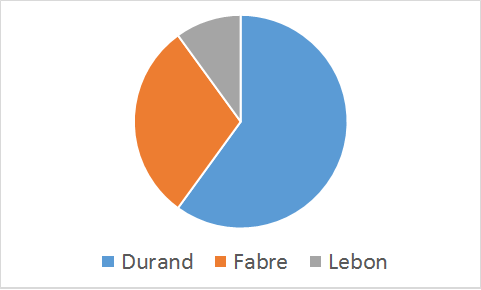
\includegraphics[scale=0.8]{img/sect1}
	\end{multicols*}
	
\end{myex}



\subsection{Diagramme en bâtons}

\begin{mybox}
	Le \kw{diagramme en bâtons (ou en barres)} est une représentation adaptée pour une série à \kw{caractère quantitatif discret}.
	
	Chaque valeur du caractère est reportée sur l'axe des abscisses. Les effectifs sont sont reportés sur l'axe des ordonnées.
	La longueur de chaque segment vertical est proportionnelle à l'effectif $n_i$ (ou à la fréquence $f_i$).
\end{mybox}

\begin{myex}
	
	\textbf{Nombre d'enfants par maison dans un lotissement}
	
	\begin{multicols*}{2}
		
		\begin{center}
			\begin{tabular}{|@{\ }c@{\ }|@{\ }c@{\ }|}
				\hline
				Nombre d'enfants & Nombre de maison \\ \hline
				0 & 3  \\ \hline
				1 & 12 \\ \hline
				2 & 9 \\ \hline
				3 & 6 \\ \hline
			\end{tabular}
		\end{center}
		
		
		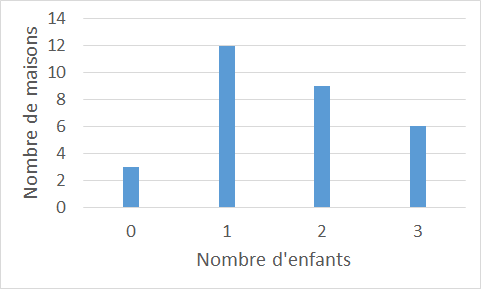
\includegraphics[scale=0.8]{img/barres}
	\end{multicols*}
	
\end{myex}



%\newpage
\subsection{Histogramme}

\begin{mybox}
	L'\kw{histogramme} est utilisé pour représenter les séries à \kw{caractère quantitatif continu}.
	
	Un histogramme est constitué d'une successions de rectangles accolés avec pour bases les amplitudes des classes $\intervFO{a}{b}$.
	Si les classes ont la même amplitude $b - a$, tous les rectangles ont la même base et les hauteurs sont proportionnelles aux effectifs $n_i$ (ou aux fréquences $f_i$).
\end{mybox}	


\begin{myex}
	
	\textbf{Hauteur des arbres dans une pépinière}
	
	\begin{multicols*}{2}
	
		\begin{center}
			\begin{tabular}{|@{\ }c@{\ }|@{\ }c@{\ }|}
				\hline
				Hauteur (en cm) & Nombre d'arbres \\ \hline
				$\intervFO{0}{100}$ & 300  \\ \hline
				$\intervFO{100}{200}$ & 150 \\ \hline
				$\intervFO{200}{300}$ & 50 \\ \hline
			\end{tabular}
		\end{center}
		
		
		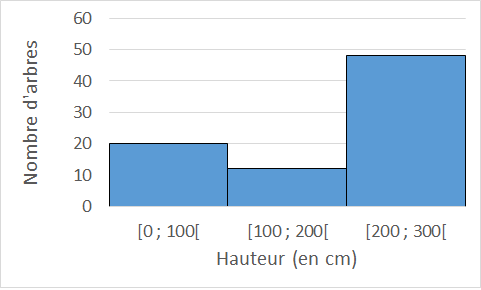
\includegraphics[scale=0.8]{img/histo}
	\end{multicols*}
	
\end{myex}



\subsection{Diagramme cartésien}

\begin{mybox}
	Le \kw{diagramme cartesien} est utilisé pour représenter l'évolution d'une grandeur par rapport à une autre (souvent le temps). 
\end{mybox}
	
\begin{myex}
	
	\textbf{\'Evolution du prix d'une baguette de pain entre 2001 et 2012}
	
	\begin{multicols*}{2}
	
		\begin{small}
			
		
		\begin{center}
			\begin{tabular}{|@{\ }c@{\ }|@{\ }c@{\ }|}
				\hline
				Année & Prix (en €) \\ \hline
				2001 & 0,66  \\ \hline
				2002 & 0,68  \\ \hline
				2003 & 0,71  \\ \hline
				2004 & 0,74  \\ \hline
				2005 & 0,75  \\ \hline
				2006 & 0,77  \\ \hline
				2007 & 0,8  \\ \hline
				2008 & 0,83  \\ \hline
%				2009 & 0,84  \\ \hline
%				2010 & 0,84  \\ \hline
%				2011 & 0,86  \\ \hline
%				2012 & 0,87  \\ \hline
			\end{tabular}
		\end{center}
		
		\end{small}	
		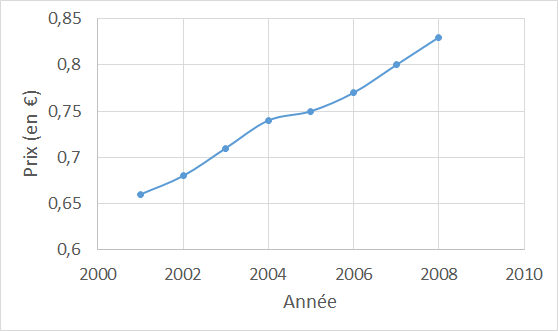
\includegraphics[scale=0.75]{img/cart}
	\end{multicols*}
	
\end{myex}

\section{Schéma récapitulatif}

\vspace*{1cm}

Le schéma ci dessous indique quel diagramme choisir pour représenter une information en fonction du type de donnée. 

\begin{center}
	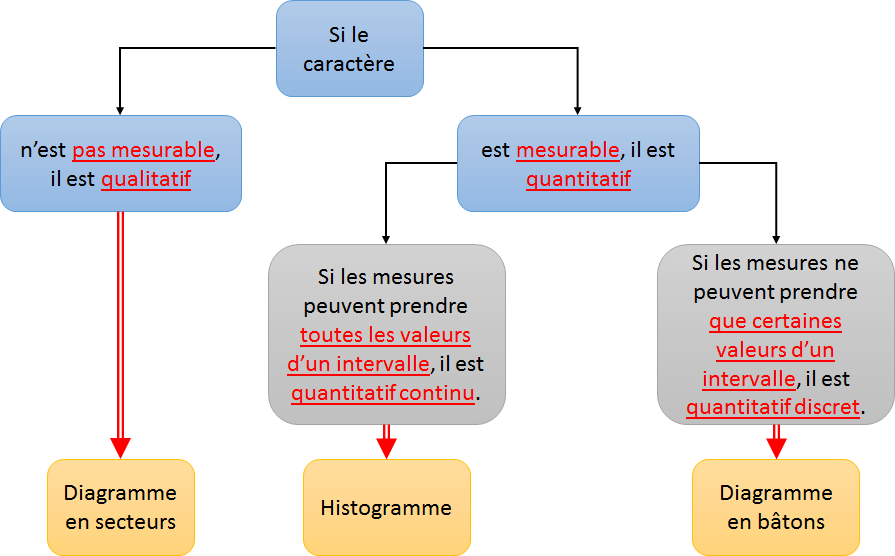
\includegraphics[scale=0.78]{img/bilan}
\end{center}
\end{document}